\chapter{Theoretical Background}\label{chap:background}

How do we locate the pose of an object in space? One way is using Electromagnetic Tracking (EMT). A magnetic field varies with position in a known way, so a sensor that measures the field carries information about where it is. The signal the sensor measures depends additionally on its orientation relative to the field, so the measurement carries information about orientation too. Current carrying coils create such a field, so a sensor in their presence can measure this generated field and locate itself.

Physics tells us how we can map from pose to measurements, a map we call the \emph{forward map}, but we want to do the opposite. We want to recover the pose given the measurements. Therefore, this is an inverse problem.

The Anser EMT system \cite{jaeger2017}, the first fully open-source EMT platform, solves exactly this problem. It infers the pose (five coordinates) of a small sensor coil from eight measurements induced by a planar array of emitter coils. 

This chapter builds the machinery needed to both understand and solve the problem. We first describe the physical system, then derive the forward map from the underlying physics. We then ask when this map can be inverted, at least locally, and turn to methods that can do this in practice.

The first class of methods we look at is the iterative methods, whose success depends on where they start. The second class is NNs, which learn an approximate inverse directly. We begin with the physical system itself.

\section{The Anser EMT System}
The Anser EMT system has two main components: a planar field generator, and a tracking sensor coil. This section describes each in turn.

\subsection{The Field Generator}
The Anser EMT system uses a planar field generator consisting of eight coils being driven at different frequencies. Each coil consists of a wound rectangular spiralling filament which first spirals inward on the top layer of a PCB, goes through a via, and then spirals back outwards on the bottom layer of the PCB, as seen in Figure \ref{fig:single_coil}. The two spiral layers together form a single coil. The coil specifications are given in Table \ref{tab:coil_spec}.

\begin{figure}
  \centering
  \includegraphics[width = 0.8\textwidth]{figs/single_coil.png} 
  \caption{Layout of a single emitter coil.}
  \label{fig:single_coil}
\end{figure}
\begin{table}
  \centering
  \begin{tabular}{ll}
    \toprule 
    Property & Value \\
    \midrule
    Outer side length & 70 \,mm \\
    Turns per coil & 25 \\
    Track width & 0.5 \, mm \\
    Track spacing & 0.25 \,mm \\
    PCB thickness & 1.6 \, mm \\
    \bottomrule
  \end{tabular}
  \caption{Specification of PCB emitter coils in Anser field generator \cite{jaeger2017}}
  \label{tab:coil_spec}
\end{table}

Eight of these coils are positioned on the PCB, as seen in Figure \ref{fig:field_coils}.
\begin{figure}
  \centering
  \includegraphics[width = 0.8 \textwidth]{figs/field_coils.png}
  \caption{Diagram of 8 emitter coils arranged as on PCB}
  \label{fig:field_coils}
\end{figure}
\subsection{The Tracking Sensor Coil}
The tracking sensor records a measurement related to the flux, and due to the emitter coils running at different frequencies, is able to recover the 8 measurements due to each of the emitter coils after demodulation. These 8 measurements are fed into the pose solving algorithm to determine the position and orientation of the sensor.

\section{Magnetic Field Derivation}
Each spiral coil is composed of a sequence of straight line filaments and Maxwell's equations in free space are linear \cite[p.~59]{griffiths2013} so the total magnetic field will be the sum of the fields of each individual straight line filament. Our main goal then, is to find the magnetic field generated at an observer point $p$ due to the current flowing along one of these straight line filaments, $\mathbf{a}$.  

We start by defining vectors $\mathbf{a}$, $\mathbf{b}$, and $\mathbf{c}$. 
\begin{itemize}
  \item $\mathbf{a}$ points along the current filament. 
  \item $\mathbf{b}$ points from the end of the filament to the observer.
  \item $\mathbf{c}$ points from the start of the filament to the observer.
\end{itemize}

Note that throughout we use the convention $\left \vert \mathbf{a} \right \vert = a$.

Now, we use the Biot Savart Law to find the magnetic field in each of the lines. 

\begin{equation*}
  \mathbf{B} = \frac{\mu_0 I}{4\pi} \int \frac{d\mathbf{l}\times \mathbf{r}}{r^3}  
\end{equation*}

To evaluate this integral we first parametrise $\mathbf{r}$ in a parameter $t$, yielding:
\begin{align*}
  \mathbf{r}(t) &= \mathbf{c} - \mathbf{a}t \text{, } t \in [0,1] \\
  d\mathbf{l} &= \mathbf{a}dt
\end{align*}

Substituting in gives:

\begin{equation*}
  \mathbf{B} = \frac{\mu_0 I}{4\pi} \int_{0}^{1} \frac{(\mathbf{a}dt)\times (\mathbf{c} - \mathbf{a}t)}{\left \vert \mathbf{c} -  t\mathbf{a}\right\vert^3}
\end{equation*}

Noting that $\mathbf{a} \times \mathbf{a} = 0$, and that $\mathbf{a}$ and $\mathbf{c}$ are constants, this simplifies to:

\begin{equation*} 
  \mathbf{B} = \frac{\mu_0 I}{4\pi}(\mathbf{a} \times \mathbf{c}) \int_{0}^{1}  \frac{dt}{\left \vert \mathbf{c} -  t\mathbf{a}\right\vert^3}
\end{equation*}

The denominator must now be simplified.
\begin{equation*}
  \left\vert \mathbf{c} - t\mathbf{a} \right \vert ^3 = \left( c^2 + t^2a^2 - 2t(\mathbf{a}\cdot \mathbf{c}) \right)^{3/2}
\end{equation*}

For simplicity, let $\beta = -(\mathbf{a} \cdot \mathbf{c})$.

\begin{equation*}
  \left\vert \mathbf{c} - t\mathbf{a} \right \vert ^3 =  \left( a^2t^2 + 2\beta t + c^2  \right)^{3/2}
\end{equation*}

Completing the square:

\begin{equation*}
  \left\vert \mathbf{c} - t\mathbf{a} \right \vert ^3 =  a^{3} \left( \left ( t + \frac{\beta}{a^2} \right)^2 -\frac{\beta^2}{a^4} + \frac{c^2}{a^2} \right)^{3/2}
\end{equation*}

Now let $u = t + \frac{\beta}{a^2}$, $du = dt$, $u(0) = \frac{\beta}{a^2}$, $u(1) = 1 + \frac{\beta}{a^2}$. Also, let $\delta = \frac{c^2}{a^2} - \frac{\beta^2}{a^4}$.

Substituting back into our Biot Savart Formula gives:

\begin{equation*}
  \mathbf{B} = \frac{\mu_0 I}{4\pi} \frac{\mathbf{a} \times \mathbf{c}}{a^3} \int_{\frac{\beta}{a^2}}^{1+\frac{\beta}{a^2}} \frac{du}{\left(u^2 + \delta\right)^{3/2}}
\end{equation*}

We want to use the identity $\sec^2\psi = 1 + \tan^2\psi$, to do so, factor out $\delta^{3/2}$

\begin{equation*}
  \mathbf{B} = \frac{\mu_0 I}{4\pi} \frac{\mathbf{a} \times \mathbf{c}}{a^3\delta^{3/2}} \int_{\frac{\beta}{a^2}}^{1+\frac{\beta}{a^2}} \frac{du}{\left(\frac{u^2}{\delta} + 1 \right)^{3/2}}
\end{equation*}

Now that it is in the correct form let: $\tan^2\psi = \frac{u^2}{\delta}$, then: 
\begin{align*}
  \tan\psi &= \frac{u}{\sqrt{\delta}} \\
  \sec^2\psi \, d\psi &= \frac{1}{\sqrt{\delta}} du \\
  \psi\left(\frac{\beta}{a^2}\right) &= \arctan \left( \frac{\beta}{a^2\sqrt{\delta}} \right) \\
  \psi\left( 1 + \frac{\beta}{a^2} \right) &= \arctan \left( \frac{1+\frac{\beta}{a^2}}{\sqrt{\delta}} \right)
\end{align*}

Substituting back in:
\begin{equation*}
  \mathbf{B} = \frac{\mu_0 I}{4\pi} \frac{\mathbf{a} \times \mathbf{c}}{a^3\delta^{3/2}} \int_{\arctan\left (\frac{\beta}{a^2\sqrt{\delta}}\right)}^{\arctan\left(\frac{1}{\sqrt{\delta}}\left(1+\frac{\beta}{a^2}\right)\right)} \frac{\sqrt{\delta} \sec^2 \psi \, d\psi}{\left(1 + \tan^2\psi \right)^{3/2}}
\end{equation*}

Using the identities $\sec^2 \psi = 1 + \tan^2 \psi$ and $\cos \psi = \frac{1}{\sec \psi}$ and simplifying yields:

\begin{equation*}
  \mathbf{B} = \frac{\mu_0 I}{4\pi} \frac{\mathbf{a} \times \mathbf{c}}{a^3\delta} \int_{\arctan\left (\frac{\beta}{a^2\sqrt{\delta}}\right)}^{\arctan\left(\frac{1}{\sqrt{\delta}}\left(1+\frac{\beta}{a^2}\right)\right)} \cos\psi \, d\psi
\end{equation*}

Solving:

\begin{equation*}
  \mathbf{B} = \frac{\mu_0 I}{4\pi} \frac{\mathbf{a} \times \mathbf{c}}{a^3\delta} \left ( \sin\left( \arctan\left(\frac{1}{\sqrt{\delta}}\left(1+\frac{\beta}{a^2}\right)\right)\right) - \sin \left( \arctan\left (\frac{\beta}{a^2\sqrt{\delta}}\right) \right) \right )
\end{equation*}

Now, we must consider a right angled triangle to work this out. $\sin\psi = \frac{o}{h}$, $\tan\psi = \frac{o}{a}$ therefore $\sin\left( \arctan \left( \frac{o}{a} \right) \right) = \frac{o}{\sqrt{o^2 + a^2}}$ by Pythagoras' Theorem.

\begin{equation*}
  \mathbf{B} = \frac{\mu_0 I}{4\pi} \frac{\mathbf{a} \times \mathbf{c}}{a^3\delta} \left( \left( \frac{1 + \frac{\beta}{a^2}}{\sqrt{\delta + \left( 1 + \frac{\beta}{a^2} \right)^2}} \right) - \left( \frac{\beta}{\sqrt{\beta^2 + a^4 \delta}} \right)  \right) 
\end{equation*}

Recalling $\delta = \frac{c^2}{a^2} - \frac{\beta^2}{a^4}$, $\beta = -\mathbf{a} \cdot \mathbf{c}$, and looking at each of the denominators:
\begin{align*}
  \sqrt{\delta + \left( 1 + \frac{\beta}{a^2} \right)^2} &= \sqrt{\frac{c^2}{a^2} - \frac{\beta^2}{a^4} + 1 + 2\frac{\beta}{a^2} + \frac{\beta^2}{a^4}} \\
                             &= \sqrt{1 + \frac{c^2}{a^2} - \frac{2}{a^2} \left(\mathbf{a} \cdot \mathbf{c} \right)} \\
                             &= \frac{1}{a} \sqrt{a^2 + c^2 - 2\left(\mathbf{a} \cdot \mathbf{c}\right)} \\
                             &= \frac{1}{a} \left \vert \mathbf{a} - \mathbf{c} \right \vert \\
                             &= \frac{b}{a}
\end{align*}

\begin{align*}
  \sqrt{\beta^2 + a^4 \delta} &= \sqrt{\beta^2 + a^2c^2 - \beta^2} \\
                              &= \sqrt{a^2c^2} \\
                              &= ac
\end{align*}

Substituting into our formula for $\mathbf{B}$ now gives:

\begin{equation*}
  \mathbf{B} = \frac{\mu_0 I}{4\pi} \frac{\mathbf{a}\times \mathbf{c}}{ac^2 - \frac{\left(\mathbf{a} \cdot \mathbf{c}\right)^2}{a}} \left( \frac{1 - \frac{\mathbf{a}\cdot{\mathbf{c}}}{a^2}}{\frac{b}{a}} + \frac{\mathbf{a} \cdot \mathbf{c}}{ac} \right)
\end{equation*}

Multiplying the numerator and denominator across by $a$

\begin{equation*}
\mathbf{B} = \frac{\mu_0 I}{4\pi} \frac{\mathbf{a}\times \mathbf{c}}{a^2c^2 - \left(\mathbf{a} \cdot \mathbf{c}\right)^2} \left( \frac{a^2 - \mathbf{a}\cdot\mathbf{c}}{b} + \frac{\mathbf{a} \cdot \mathbf{c}}{c} \right)
\end{equation*}

Now, picking out these two parts and simplifying, where $\alpha$ is the angle between $\mathbf{a}$ and $\mathbf{c}$:
\begin{align*}
  a^2c^2 - \left( \mathbf{a} \cdot \mathbf{c} \right)^2 &= a^2c^2 - a^2c^2\cos^2(\alpha) \\
                               &= a^2c^2(1 - \cos^2\alpha) \\
                               &= a^2c^2\sin^2\alpha \\
                               &= \left \vert \mathbf{a} \times \mathbf{c} \right \vert ^2
\end{align*}
\begin{align*}
  a^2 - \mathbf{a} \cdot \mathbf{c} &= \mathbf{a} \cdot \mathbf{a} - \mathbf{a} \cdot \mathbf{c} \\
                              &= \mathbf{a} \cdot \left(\mathbf{a} - \mathbf{c}\right) \\
                              &= \mathbf{a} \cdot (-\mathbf{b}) \\
                              &= - \mathbf{a} \cdot \mathbf{b}
\end{align*}
This gives us our final form:
\begin{equation}\label{eq:biot_savart_final}
  \mathbf{B} = \frac{\mu_0 I}{4\pi} \frac{\mathbf{a} \times \mathbf{c}}{\left \vert \mathbf{a} \times \mathbf{c} \right \vert^2 } \left( \frac{\mathbf{a} \cdot \mathbf{c}}{c} - \frac{\mathbf{a} \cdot \mathbf{b}}{b} \right)
\end{equation}
Now, remembering that this equation is linear and that each coil is made up of straight line filaments we get:

\begin{equation*}
\mathbf{B}_{\text{total}} = \sum_{\text{coils}} \sum_{\text{filaments}}  \mathbf{B}_{\text{filament}} 
\end{equation*}
Now, since we are in free space we use the identity $\mathbf{H} = \frac{\mathbf{B}}{\mu_0}$ \cite[p.~285]{griffiths2013}

\section{Understanding the forward map}\label{sec:forward-map}
The problem is framed as an inverse problem. The forward map takes position and orientation data and calculates 8 measurements from each of the coils. Our goal is to approximate an inverse to this map. To do so, we first try to understand the forward map. 
\subsection{Definition and properties}
First we define a pose vector $\mathbf{p} \in \mathbb{R}^5$ 
\begin{equation}
  \mathbf{p} = 
  \begin{bmatrix}
    x \\ y \\ z \\ \theta \\ \phi 
  \end{bmatrix}
\end{equation}

In practice, $\mathbf{p}$ is restricted to a set $\Omega \subset \mathbb{R}^5$

\begin{equation}
  \Omega = \left\{
  \begin{bmatrix} x \\ y \\ z \\ \theta \\ \phi \end{bmatrix} \in \mathbb{R}^5 : 
  \begin{matrix} x \in (-0.125\text{ m},0.125\text{ m}) \\ y \in (-0.125\text{ m},0.125\text{ m}) \\ z \in (0.0016 \text{ m},0.25\text{ m}) \\ \theta \in (0\text{ rad},\pi\text{ rad}) \\ \phi \in [0\text{ rad},2\pi\text{ rad}) \end{matrix}
  \right\}
\end{equation}

Then we define a vector of measurements, $\mathbf{m} \in \mathbb{R}^8$
\begin{equation}
  \mathbf{m} = 
  \begin{bmatrix}
    m_1 \\ m_2 \\ m_3 \\ m_4 \\ m_5 \\ m_6 \\ m_7 \\ m_8 
  \end{bmatrix}
\end{equation}

Now we can write the forward map: $\mathbf{F}(\mathbf{p}): \Omega \subset \mathbb{R}^5 \rightarrow \mathbb{R}^8$. More precisely,
\begin{equation}
  m_i = \mathbf{H}_i(x,y,z) \cdot \hat{n}(\theta,\phi) 
  \label{eq:forward}
\end{equation}
where $\mathbf{H}_i$ is the magnetic field calculated at $(x,y,z)$ due to coil $i$ using equation \eqref{eq:biot_savart_final}, and $\hat{n}(\theta,\phi)$ is the vector normal to the sensor, defined by: 

\begin{equation}
  \hat{n}(\theta,\phi) = 
  \begin{bmatrix}
    \sin\theta\cos\phi \\ \sin\theta\sin\phi \\ \cos\theta
  \end{bmatrix}
\end{equation}
Since $F$ is smooth, the image of the 5-dimensional domain, $\Omega$, has measure zero in $\mathbb{R}^8$, therefore $F$ cannot be surjective.

\subsection{The Jacobian}
Now that we have established that $F$ is not surjective we must move our attention to thinking about local invertibility rather than global. To do so we make a local approximation:
\begin{equation}
  F(\mathbf{p} + \mathbf{\delta}) = F(\mathbf{p}) + J(\mathbf{p})\mathbf{\delta}
\end{equation}
where $\boldsymbol{delta}$ is a small step in $\mathbb{R}^5$, and $J$ is the \emph{Jacobian}, defined by:
Jacobian:
\begin{definition}[Jacobian]
  $$ J(\mathbf{p}) = \frac{\partial F}{\partial \mathbf{p}} \in \mathbb{R}^{8\times5} \text{, } J_{i,j} = \frac{\partial F_i}{\partial p_j} $$
\end{definition}
$\mathbf{H}$ is a smooth map away from the current filaments. $\hat{n}$ is also a smooth map, therefore $F$ will also be smooth away from the plane of the field generator and the Jacobian will be well defined there.

A closed form for $\mathbf{J}$ is cumbersome to find so we instead use finite differences to approximate $\mathbf{J}$

\begin{equation}\label{eq:jacobian}
\mathbf{J_{:,i}} \approx \frac{F\left(\mathbf{p} + h  \hat{e_i} \right) - F(\mathbf{p})}{h}
\end{equation}
where $\hat{e}_i$ is the unit vector in the $i$th direction, and $h$ is a small real value.

\subsection{Local Invertibility}
The forward map sends $\Omega \subset \mathbb{R}^5$ into $\mathbb{R}^8$, so it is never
globally invertible. This raises the question: when, if ever, is the forward map
locally invertible?

The derivative of $F$ at a point $\mathbf{p}_0 \in \Omega$ is the linear map
$J_0 = J(\mathbf{p}_0) \in \mathbb{R}^{8 \times 5}$. The following conditions are
equivalent:
$$
  J_0^\top J_0 \text{ invertible}
  \iff J_0 \text{ has full column rank}
  \iff J_0 \text{ is injective as a linear map.}
$$
It can be shown \cite{mckay2022} that if $J_0$ has full column rank, then $F$ is
injective on a neighbourhood of $\mathbf{p}_0$. This means that the pose is unique
in that neighbourhood: distinct nearby poses produce distinct measurements, and the
pose is locally recoverable from the measurement. As we will see later, in Section \ref{sec:GN}, $J^\top J$ is exactly the matrix the Gauss-Newton algorithm must invert. 

Rank deficiency therefore signals regions where the pose cannot be recovered from
the measurement, even locally. Full column rank is a condition for the inverse
problem to be well posed.

\section{Iterative Methods}
Given a function $f : \mathbb{R}^n \rightarrow \mathbb{R}^m$ with $m \geq n$, and a given $y \in \mathbb{R}^m$ suppose we want to find an $x \in \mathbb{R}^n$ that satisfies $y = f(x)$. In the case $m = n$ we could get bijectivity which would allow us to simply invert the map, however, in our case we have $n = 5$ and $m = 8$ so we cannot. This leads us to iterative methods.

\subsection{Gauss-Newton}\label{sec:GN}
The Gauss-Newton (GN) Algorithm \cite{nocedal2006} solves this exact kind of problem. 

We have a function $f : \mathbb{R}^n \rightarrow \mathbb{R}^m$ and we know $y \in \mathbb{R}^m$, we want to find $x_{\text{true}} \in \mathbb{R}^n$ such that $y = f(x_{\text{true}})$. We start with an initial guess $x_0 \in \mathbb{R}^n$ and define a residual:
\begin{equation}
  r(x) = f(x) - y
\end{equation}
Then we define a cost function: 
\begin{equation}
  C(x) = \frac{1}{2} \left \Vert r(x) \right \Vert^2 = \frac{1}{2} r(x)^{\top}r(x)
  \label{eq:cost_function}
\end{equation}
Suppose now we take a step, $\delta \in \mathbb{R}^n$, we want to find the $\delta$ which minimises the cost function.
\begin{equation}
  C(x + \delta) = \frac{1}{2} \left\Vert r(x + \delta) \right\Vert^2 
\end{equation}
Now, linearising:
\begin{equation}
  C(x + \delta) \approx \frac{1}{2} \left\Vert r(x) + J(x)\delta \right\Vert^2 
\end{equation}
Since this is a scalar quantity we can take $\nabla_\delta C$ and set it to zero to find the minimum.
\begin{equation}
  \nabla_\delta C(x + \delta) = \left(\frac{\partial}{\partial \delta} C(x + \delta)\right)^\top = 0
\end{equation}
Now, we consider the $k$th component of this gradient:
\begin{align}
  \left(\nabla_\delta C(x + \delta)\right)_k
    &\approx \frac{1}{2}\frac{\partial}{\partial \delta_k} \sum_{j = 1}^{m} \left(r_j(x) + \sum_{i=1}^n J_{ji}(x)\delta_i \right)^2 \\
    &\approx \frac{1}{2} \sum_{j = 1}^m 2\left(r_j(x) + \sum_{i=1}^n J_{ji}(x)\delta_i\right)\frac{\partial}{\partial \delta_k}\left(r_j(x) + \sum_{i=1}^n J_{ji}(x)\delta_i\right) \\
    &\approx \sum_{j = 1}^m J_{jk}(x)\left(r_j(x) + \sum_{i=1}^n J_{ji}(x)\delta_i\right) \\
    &\approx \sum_{j = 1}^m J_{jk} r_j + \sum_{j = 1}^m \sum_{i=1}^n J_{jk} J_{ji}\delta_i \\
    &\approx \left( J^\top r \right)_k + (J^\top J \delta)_k
\end{align}
Since this applies for all $k$ we get:
\begin{equation}
  \nabla_\delta C(x + \delta) \approx J^\top r + J^\top J \delta
\end{equation}
Setting this equal to zero and solving, yields:
\begin{equation}
  \delta = -\left(J^\top J\right)^{-1} J^\top r 
\end{equation}
Now that we know the theoretically "best" step to take, we iterate and do this repeatedly:
\begin{equation}
  x_{i + 1} = x_i - \left(J(x_i)^\top J(x_i)\right)^{-1}J(x_i)^\top r(x_i)
\end{equation}

This method has a known failure mode: it has no step-size control. Far from the solution, where the linearisation is poor, the full step can increase the cost and the iteration can diverge.
\subsection{Gradient Methods}
Gauss-Newton fails when it "trusts" the linear model too far from the point at which it was linearised. The opposite approach makes no model of the residual at all. It just moves in the direction that decreases the cost the fastest. Consider the cost function \eqref{eq:cost_function} and take its gradient.
\begin{equation}
  \nabla_x C(x) = \nabla_x \frac{1}{2} r(x)^\top r(x)
\end{equation}
Using the same argument as before, taking the $k$th component of this gradient:
\begin{align}
  \left(\nabla_x C(x)\right)_k &= \frac{1}{2} \frac{\partial}{\partial x_k} \sum_{j = 1}^{m} r_j(x) r_j(x) \\
                &= \frac{1}{2} \sum_{j = 1}^{m} \frac{\partial}{\partial x_k} r_j(x)^2 \\
                &= \frac{1}{2} \sum_{j = 1}^m 2r_j(x) \frac{\partial r_j(x)}{\partial x_k} \\
                &= \sum_{j = 1}^m r_j(x) \frac{\partial (f_j(x) - y_j)}{\partial x_k} \\
                &= \sum_{j = 1}^m r_j(x) \frac{\partial f_j(x)}{\partial x_k} \\
                &= \sum_{j=1}^m r_j(x) J_{jk}(x) \\
                &= \left(J^\top(x) r(x)\right)_k
\end{align}
Gradient descent then steps against this gradient, with the step-size being denoted by the parameter $\eta \in \mathbb{R}$:
\begin{equation}
  x_{i + 1} = x_i - \eta J(x_i)^\top r(x_i) 
\end{equation}
Because $-\nabla_x C$ is in the direction of steepest local decrease, a sufficiently small $\eta$ is guaranteed to reduce the cost, so the method is robust far from the solution where Gauss-Newton diverges. Its failure mode is also the opposite of Gauss-Newton's. Near the solution, the gradient becomes small, and since the algorithm has no knowledge of the distance to the solution it bounces back and forth around the minimum.

\subsection{Levenberg's Contribution}\label{sec:background-lm}
In 1944, Levenberg \cite{levenberg1944} interpolated between these two algorithms. If we denote each step as $\delta_{GN}$ and $\delta_{GD}$, for Gauss-Newton and gradient descent, respectively we get that each of these steps solves the equations:
\begin{align}
  (J^\top J) \delta_{GN} &= - J^\top r \\
  \delta_{GD} &= -\eta J^\top r
\end{align}
Now, letting $\lambda = \frac{1}{\eta}$, multiplying by $I \in \mathbb{R}^{n \times n}$, and interpolating between these two yields:
\begin{equation}
  \label{eq:levenberg}
  \left(J^\top J + \lambda I \right)\delta = -J^\top r
\end{equation}
Here, $\lambda$ is known as the damping factor, and another key insight Levenberg had was to vary $\lambda$. Since GN works better the closer to the solution we get and GD works better the further from the solution we are, the damping is varied dynamically.\\
We start at step $i$ with $\lambda = \lambda_i$. If $C(x_{i+1}) < C(x_i)$ we are moving in the right direction so can move more into the GN regime, setting $\lambda_{i+1} = 0.1\lambda_i$. However, if $C(x_{i+1}) \geq C(x_{i})$ then it is clear that GN is not working and we need to move into a GD dominated regime, thus setting $\lambda_{i+1} = 10\lambda_{i}$. This ensures that when we are far from the solution we are in a GD dominated regime and as we get closer to the solution GN starts to take over.

\subsection{The Levenberg Marquardt Algorithm} 
One downfall of Levenberg's approach is that $\lambda$ is the same in every dimension, even though the dimensions may operate on different scales. Marquardt \cite{marquardt1963} solves this by replacing the identity matrix, $I$ with  $D = \operatorname{Diag}\left(J^\top J\right)$ to scale the weights, where $\operatorname{Diag}$ is the operator which acts on matrices by setting the off-diagonal elements to zero and operates on vectors by making a diagonal matrix out of its components. The Levenberg-Marquardt algorithm solves the following equation at every iteration:
\begin{equation}
  \label{eq:lm}
  \left(J^{\top}J + \lambda D \right)\delta = -J^{\top} r 
\end{equation}
This means that the algorithm works with different damping in each direction, proportional to the "scale" of that particular direction.

\subsection{Convergence and the Role of Initialisation}
Both Gauss-Newton and LM are local methods: they converge to a stationary point of $C$, and which stationary point depends on where they start. Since $C$ is typically non-convex it can have multiple local minima, an example is shown in Figure \ref{fig:local_minima}. In our problem, in particular, given the high levels of symmetry between the coils, it is highly likely that there are multiple minima. These iterative methods work when the initial guess is in the correct basin of attraction. That then raises the question, how do we get into the right basin of attraction?
\begin{figure}
  \centering
  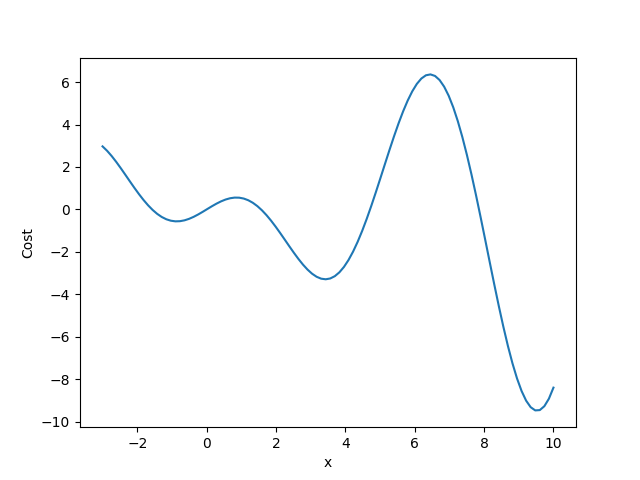
\includegraphics[width=0.8\textwidth]{figs/local_minima.png}
  \caption{Example showing multiple local minima using $y = x\cos x$, $x \in (-3,10)$}
  \label{fig:local_minima}
\end{figure}
\section{Neural Networks for learning inverses}
The iterative methods above invert the forward map each time for every measurement. An alternative would be to spend the computation time upfront and approximate a full inverse map once.

\subsection{Feed Forward Neural Network}
We use a fully-connected feed forward NN to approximate the inverse. Suppose we have a function $F: \mathbb{R}^N \rightarrow \mathbb{R}^M$ an approximate inverse is defined on the image of $F$, which we call $\hat{F}^{-1}$. We would like to find $y \in \mathbb{R}^N$ such that $y = \hat{F}^{-1}(x), x \in \mathbb{R}^M$. To do so, a feed-forward NN with $L$ hidden layers performs the composition shown in equation \eqref{eq:FFNN}, with $o_0 = x$ and $o_L = \hat{y}$:

\begin{align}
  \label{eq:FFNN}
  o_{i+1} &= \sigma \left(W_io_i + b_i\right) \text{,} i \in \{0,1,2,...l-2\} \\ 
  o_{L} &= W_{L-1}o_{l+1} + b_{l-1}
\end{align}
where $W_i$ and $b_i$ are the weight matrices and bias vectors (collectively the parameters $w$), and $\sigma$ is the nonlinear activation function.
We represent this approximation as $\hat{F}^{-1}_w: \mathbb{R}^M \rightarrow \mathbb{R}^N$, with $\hat{y} = \hat{F}^{-1}_w(x)$ 

The question then becomes how do we find the collection of parameters, $w$, which does this?

\subsection{Training a Neural Network}
Because we possess $F$ we can generate unlimited training data, a collection of labelled pairs, $(x_i,y_i)$. The goal of training is then to minimise the \emph{loss function} with respect to the parameters, $w$. The loss function is a performance metric for the network, and we will see in Section \ref{sec:res-network} that the choice of loss function is crucial to make a network perform well.
We minimise the loss using an optimiser, in our case the Adam optimiser \cite{kingma2017}. Generalisation is then assessed on a held-out test set never seen during training.
